\section{Results}
\label{sec:results}

In the following, the molar heat capacity and then the Debye temperature are determined.

\subsection{Parameters}
\label{sec:parameters}

The copper sample in this experiment has a mass of $m = \qty{0.342}{\kilo\gram}$ \textnormal{\cite{molar_heat}} and a density of
$ \rho = \qty{8930}{\kilo\gram \per \meter^3 }$ \textnormal{\cite{kupfer}}.
The table \ref{tab:parameters} shows the molar volume and the compression modul of copper.
%erstelle tabelle
\begin{table}[H]
	\centering
	\caption{Parameters of the copper sample}
	\label{tab:parameters}
	\begin{tabular}{c c }
		\toprule
		Parameter & Value \\
		\midrule
		$V_m$ & $\qty{7.11e-6}{\meter^3 \per \mol}$ \cite{chemie_kupfer}\\
		$\kappa$ & $\qty{140} {\giga\pascal}$ \cite{perioden_kupfer}\\
		\bottomrule
	\end{tabular}
\end{table}

The molar mass, the number of moles and the number of particles can then be calculated.
The following applies to the molar mass
\begin{equation*}
	M = V_m \cdot \rho = \qty{0.0634}{\kilo\gram \per \mol}.
\end{equation*}

The number of moles is calculated as follows
\begin{equation*}
	n = \frac{m}{M} = \num{5.103}
\end{equation*}

The result for the number of particles is
\begin{equation*}
	N = n \cdot N_A = \num{3.07e24}.
\end{equation*}

The volume of the sample is calculated as follows
\begin{equation*}
	V = \frac{m}{\rho} = \qty{3.628e-5}{\meter^3}.
\end{equation*}

The transverse velocity of sound and the longitudinal velocity of sound are also required for further calculations.
These are $v_t = \qty{2260}{\meter \per \second}$ and $v_l = \qty{4700}{\meter \per \second}$ \cite{molar_heat}.

\subsection{Theoretical Debye Temperature}
\label{sec:theoretical_debye_temperature}

The Debye temperature is calculated using the formula \ref{eqn:debye_temperature}.
The Debye frequency is determined by the formula \ref{eqn:debye_frequency}.
The result for the Debye temperature with the parameters given in section \ref{sec:parameters} is
\begin{equation*}
	\vartheta_D = \qty{332.208}{\kelvin}.
\end{equation*}


\subsection{Calculation of the Molar Heat Capacity Cp}
\label{sec:calculation_of_the_molar_heat_capacity_cp}

The molar heat capacity $C_{\text{P}}$ can be calculated using the equation
\begin{equation}
	C_{\text{P}} = \frac{1}{n} \cdot \frac{E}{\Delta T}.
\end{equation}
Here the energy is defined as follows
\begin{equation}
	E = I \cdot U \cdot \Delta t.
\end{equation}

The calculated heat capacity's are shown in Table \ref{tab:heat_capacity1}.

\begin{table}[H]
	\centering
	\caption{Temperature difference $\Delta T$, time intervall $\Delta t$, voltage $U$, current $I$ and the molar heat capacity $C_{\text{P}}$}
	\label{tab:heat_capacity1}
	\begin{tabular}{c c c c c c}
	\toprule
	$\Delta T / \unit{\kelvin}$ & $\Delta t / \unit{\second}$ & $U / \unit{\volt} $ & $I / \unit{\milli\ampere}$ & $C_{\text{P}} / \unit{\joule\per\kelvin\per\mol}$ \\
	\midrule
	\num{11.87+-0.34}& \num{382+-7.07}& \num{17.20+-0.01} & \num{164.1} & \num{12.40+-7.57} \\
	\num{10.02+-0.34}& \num{336+-7.07}& \num{17.37+-0.01} & \num{165.4} & \num{21.47+-13.0} \\
	\num{10.07+-0.34}& \num{340+-7.07}& \num{17.45+-0.01} & \num{166.0} & \num{18.95+-11.44} \\
	\num{9.87+-0.34}& \num{356+-7.07}& \num{17.52+-0.01} & \num{166.4} & \num{19.68+-11.85} \\
	\num{9.92+-0.34}& \num{350+-7.07}& \num{17.57+-0.01} & \num{166.8} & \num{20.62+-12.39} \\
	\num{9.96+-0.34}& \num{377+-7.07}& \num{17.61+-0.01} & \num{167.0} & \num{20.25+-12.15} \\
	\num{10.01+-0.35}& \num{377+-7.07}& \num{17.64+-0.01} & \num{167.3} & \num{21.79+-13.05} \\
	\num{10.05+-0.35}& \num{383+-7.07}& \num{17.67+-0.01} & \num{167.4} & \num{22.08+-13.22} \\
	\num{10.10+-0.35}& \num{384+-7.07}& \num{17.69+-0.01} & \num{167.6} & \num{22.09+-13.21} \\
	\num{10.14+-0.35}& \num{415+-7.07}& \num{17.71+-0.01} & \num{167.7} & \num{23.81+-14.23} \\
	\num{9.69+-0.35}& \num{373+-7.07}& \num{17.72+-0.01} & \num{167.8} & \num{22.43+-13.4} \\
	\num{9.98+-0.35}& \num{386+-7.07}& \num{17.73+-0.01} & \num{167.9} & \num{22.56+-13.47} \\
	\num{10.02+-0.35}& \num{408+-7.07}& \num{17.74+-0.01} & \num{168.0} & \num{23.77+-14.18} \\
	\num{9.81+-0.36}& \num{400+-7.07}& \num{17.75+-0.01} & \num{168.0} & \num{23.82+-14.21} \\
	\num{10.11+-0.36}& \num{450+-7.07}& \num{17.75+-0.01} & \num{168.1} & \num{26.03+-15.52} \\
	\num{9.90+-0.36}& \num{422+-7.07}& \num{17.76+-0.01} & \num{168.2} & \num{24.96+-14.87} \\
	\num{10.19+-0.36}& \num{392+-7.07}& \num{17.76+-0.01} & \num{168.2} & \num{22.51+-13.41} \\
	\num{9.98+-0.36}& \num{420+-7.07}& \num{17.76+-0.01} & \num{168.3} & \num{24.65+-14.68} \\
	\bottomrule
		\end{tabular}
\end{table}

\subsection{Calculation of the Molar Heat Capacity $C_{\text{V}}$}
\label{sec:calculation_of_the_molar_heat_capacity_cv}

The molar heat capacity $C_{\text{V}}$ can be calculated using the equation \ref{eqn:heat_capacity_difference}.
The values of the expansion coefficient can be read from the Figure \ref{fig:expansion}.
The heat capacities, the temperatures and the expansion coefficient are shown in Figure .

\begin{table}[H]
	\centering
	\caption{Tempearture $T$, heat capacity $C_{\text{V}}$ and expansion coefficient $\alpha$}
	\begin{tabular}{c c c}
	\toprule
	$T / \unit{\kelvin}$ & $C_{\text{V}} / \unit{\joule\per\kelvin\per\mol}$ & $\alpha $\\
	\midrule
	\num{91.44+-0.24}& \num{12.32+-7.57}& \num{9.75e-06} \\
	\num{103.31+-0.24}& \num{21.36+-13.0}& \num{1.07e-05} \\
	\num{113.33+-0.24}& \num{18.82+-11.44}& \num{1.15e-05} \\
	\num{123.39+-0.24}& \num{19.52+-11.85}& \num{1.21e-05} \\
	\num{133.27+-0.24}& \num{20.43+-12.39}& \num{1.265e-05} \\
	\num{143.18+-0.24}& \num{20.03+-12.15}& \num{1.315e-05} \\
	\num{153.15+-0.24}& \num{21.54+-13.05}& \num{1.36e-05} \\
	\num{163.15+-0.24}& \num{21.81+-13.22}& \num{1.39e-05} \\
	\num{173.21+-0.25}& \num{21.79+-13.21}& \num{1.425e-05} \\
	\num{183.3+-0.25}& \num{23.48+-14.23}& \num{1.45e-05} \\
	\num{193.45+-0.25}& \num{22.06+-13.4}& \num{1.475e-05} \\
	\num{203.14+-0.25}& \num{22.16+-13.47}& \num{1.495e-05} \\
	\num{213.12+-0.25}& \num{23.34+-14.18}& \num{1.52e-05} \\
	\num{223.14+-0.25}& \num{23.35+-14.21}& \num{1.54e-05} \\
	\num{232.95+-0.25}& \num{25.53+-15.52}& \num{1.56e-05} \\
	\num{243.06+-0.25}& \num{24.43+-14.87}& \num{1.575e-05} \\
	\num{252.96+-0.25}& \num{21.95+-13.41}& \num{1.59e-05} \\
	\num{263.15+-0.26}& \num{24.05+-14.68}& \num{1.610e-05} \\
	\num{273.13+-0.26}& \num{24.05+-14.68}& \num{1.625e-05} \\
	\bottomrule
	\end{tabular}
\end{table}

The calculated heat capacity values were plotted as a function of temperature in plot \ref{fig:heat_capacity_plot}.

\begin{figure}[H]
	\centering
	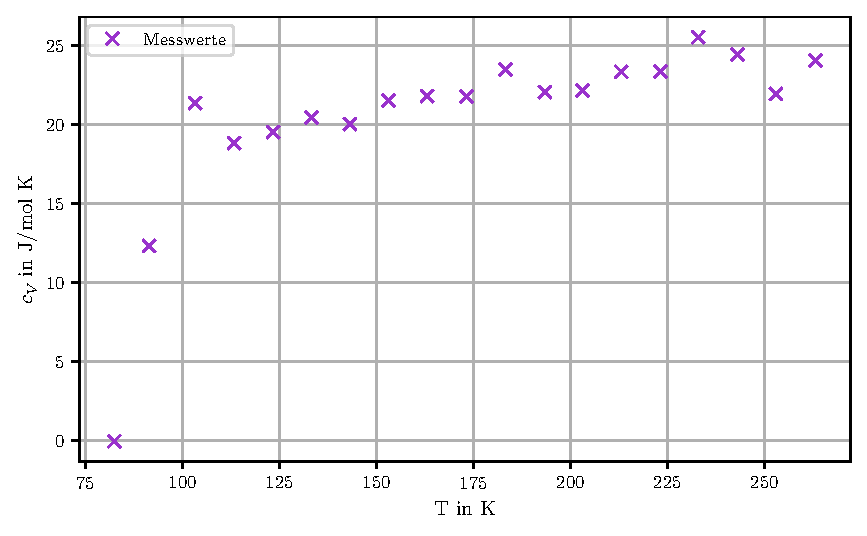
\includegraphics[width=0.7\textwidth]{build/Cv.pdf}
	\caption{The molar heat capacity $C_{\text{V}}$ as a function of temperature}
	\label{fig:heat_capacity_plot}
\end{figure}

\subsection{Experimental Debye Temperature}
\label{sec:experimental_debye_temperature}

With the help of the table \ref{fig:ratio}, the Debye temperature per temperature can be determined by reading
the calculated values from our $C_{\text{V}}$ and then assigning them.
Then only the quotient $\frac{\vartheta_D}{T}$ has to be multiplied by the temperature $T$ to obtain the Debye temperature $\vartheta_D$.
Values can only be calculated for temperatures below \qty{170}{\kelvin}.

The calculated Debye temperatures are shown in Table \ref{tab:debye_temperature}.

\begin{table}[H]
	\centering
	\caption{Temperature $T$, Debye temperature $\vartheta_D$}
	\label{tab:debye_temperature}
	\begin{tabular}{c c}
	\toprule
	$T / \unit{\kelvin}$ & $\vartheta_D / \unit{\kelvin}$ \\
	\midrule
	\num{91.44+-0.24}& \num{338.1+-1.0} \\
	\num{103.31+-0.24}& \num{258.3+-0.6} \\
	\num{113.33+-0.24}& \num{260.7+-0.5} \\
	\num{123.39+-0.24}& \num{246.8+-0.5} \\
	\num{133.27+-0.24}& \num{293.2+-0.5} \\
	\num{143.18+-0.24}& \num{386.6+-0.7} \\
	\num{153.15+-0.24}& \num{413.5+-0.7} \\
	\num{163.15+-0.24}& \num{440.5+-0.7} \\
	\bottomrule
	\end{tabular}
\end{table}

The mean value of the Debye temperatures is $\qty{299.27+-0.19}{\kelvin}$.
